\title{Gallery of single layer textures}

Can a single-layer convolutional neural network hallucinate snowflakes when
given white noise as input?  The answer is {\bf yes}.

Here we show a gallery of textures created by such ``single layer CNN''.

More precisely,
the basic construction depends on three functions:
\begin{enumerate}
	\item $f$ a probability density on~$\mathbf{R}$
	\item $g\in L^1_{loc}(\mathbf{R^2})$ a convolution kernel on the plane
	\item $h:\mathbf{R}\to[0,255]$ a monotonic tone mapping
\end{enumerate}
%~$f$ (a probability density
%on~$\mathbf{R}$), $g\in L^1_{loc}(\mathbf{R^2})$ and~$h:\mathbf{R}\to[0,255]$.
To generate a random texture~$I$, run the following algorithm
\begin{enumerate}
	\item Build a white noise image~$n$ of distribution~$f$.
	\item Compute~$I=h\circ (g*n)$
\end{enumerate}
The function~$h$ is chosen to transport the histogram of~$g*n$
into~$[0,255]$.  For example, a simplest color balance or an Otsu
thresholding.  The kernel~$g$ is typically positive and radial, or a
derivative of a radial function.


\emph{Note:}
This is a fully reproducible document.
Each greyed-out section is the complete script used to produce the
corresponding image.  All of them are drawings over a blank canvas of
arbitrary size:

%RUN_VERBATIMS sh &
\begin{verbatim}
plambda zero:768x768 "" -o canvas;
\end{verbatim}

For numerical reasons, especially with non-positive kernels, some of the
computations are performed in the frequency domain.  Thus, sometimes it may
not be evident that there is a single linear filter.  But all the textures in
this page are indeed single-layer.

\section{Binary}
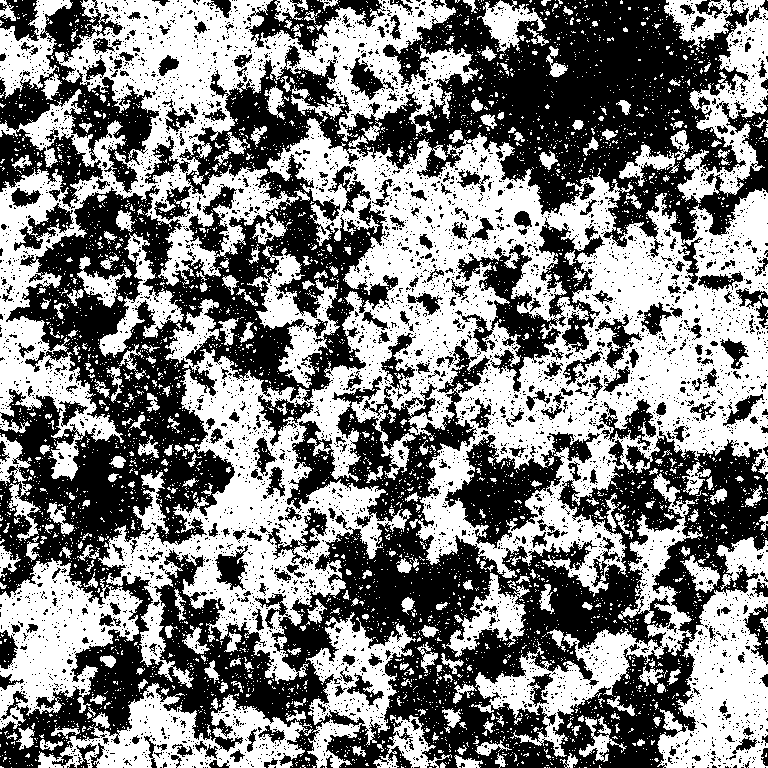
\includegraphics{binary.png}
\begin{verbatim}
plambda canvas randc | blur c 0.5 | plambda - 'x x%m > 255 *' -o binary.png
\end{verbatim}
Comment: this is Cauchy white noise blurred with a Cauchy kernel, binarized
at the median value.

\section{Disks}
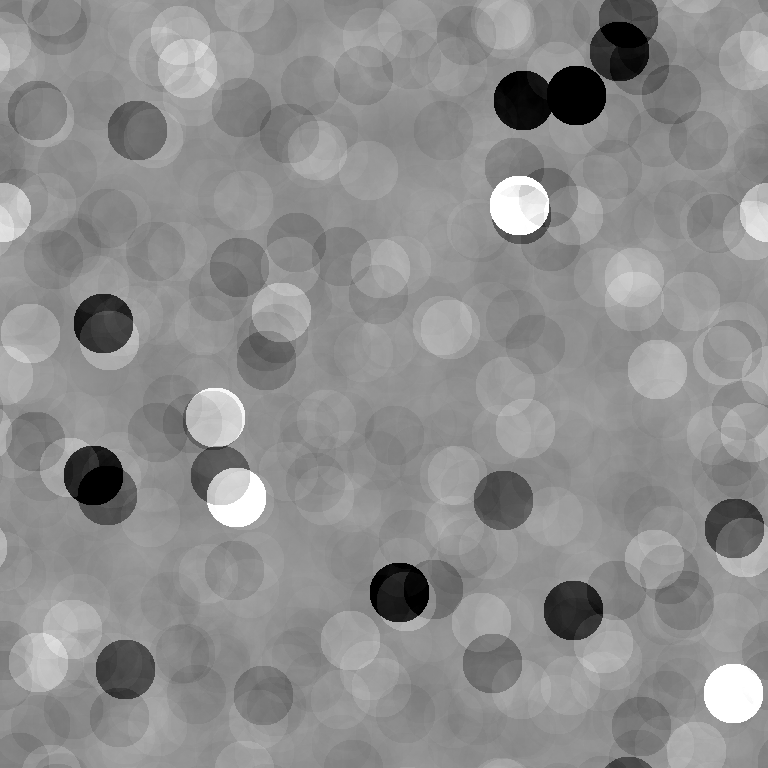
\includegraphics{disks.png}
\begin{verbatim}
plambda canvas randc | blur disk 30 | qauto -p 1 - disks.png
\end{verbatim}
Comment: This is Cauchy white noise blurred with a circular kernel, followed
by a simplest color balance that saturates~$1\%$ of the pixels.

\section{Starfield}
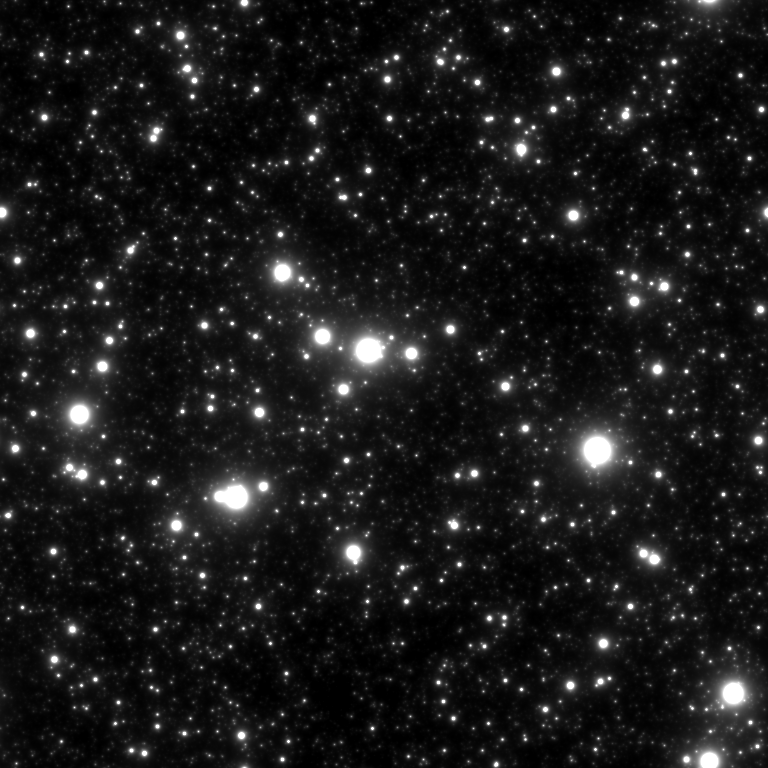
\includegraphics{starfield.png}
\begin{verbatim}
plambda canvas randp | blur c 1 | qauto -p 1 - starfield.png
\end{verbatim}
Comment: This is Pareto white noise blurred with a Cauchy kernel, followed by
a simplest color balance that saturates~$1\%$ of the pixels.

\section{Blood}

\includegraphics{blood.png}
\begin{verbatim}
SIGMOID='2 * tanh 1 + 2 /'
RED='dup 1 rot - rot 1 1 1 join3 * 0.7 0.1 0.1 join3 * + 255 *'
plambda canvas randp|blur c 1|plambda - "x x%O80 - $SIGMOID $RED" -o blood.png
\end{verbatim}
Comment: this is exactly the same image as \verb+starfield.png+, but with a
red palette.

\section{Islands}
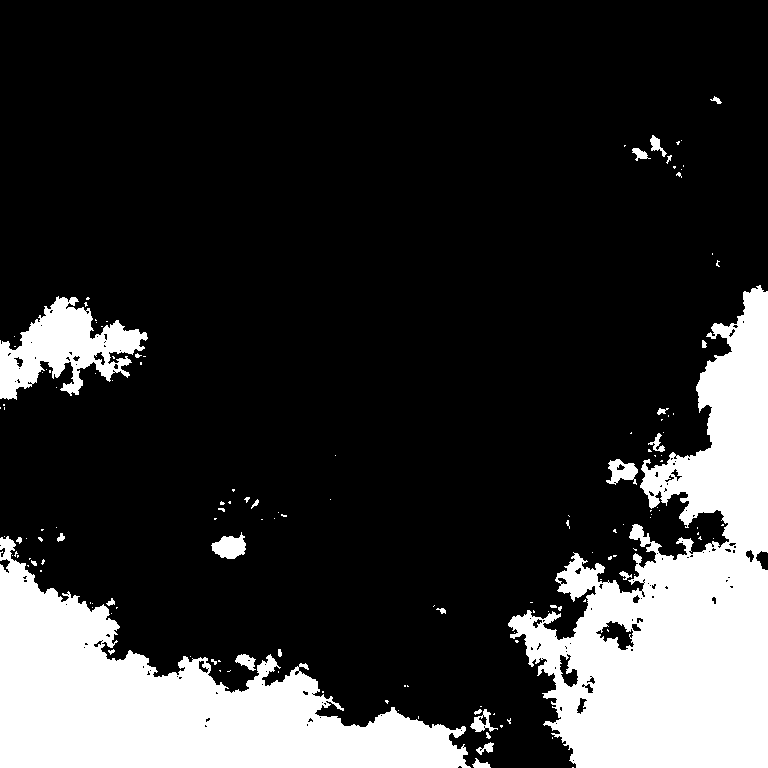
\includegraphics{islands.png}
\begin{verbatim}
plambda canvas randu | blur -s z .4 | plambda - 'x x%O80 > 255 *' -o islands.png
\end{verbatim}
Comment: uniform white noise, blurred by a kernel of the form~$1/\log(r)$,
binarized to the 80th quantile.


\section{Clouds}
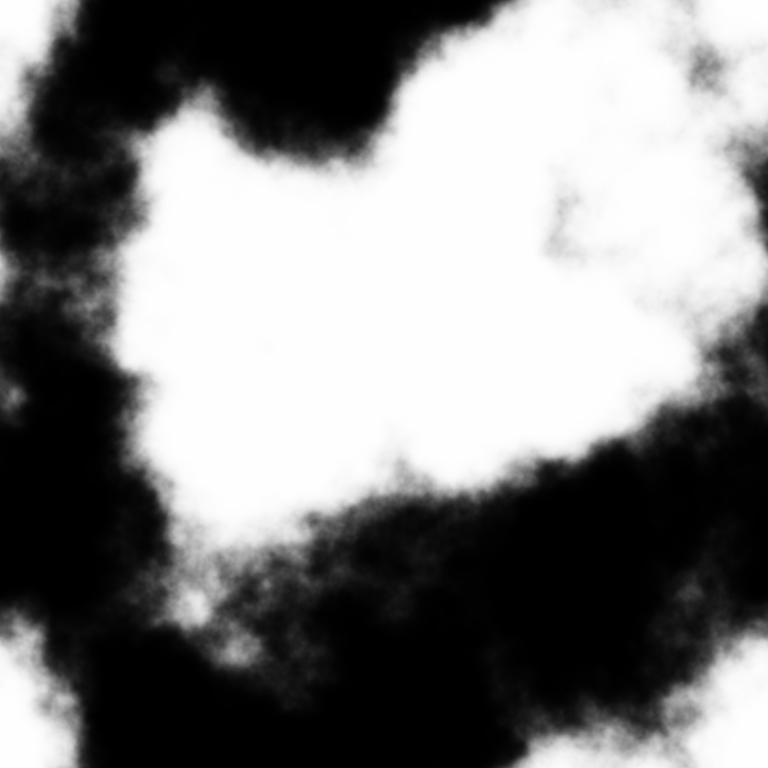
\includegraphics{clouds.png}
\begin{verbatim}
SIGMOID='4e4 * tanh 1 + 2 /'
BLUE='dup 1 - -1 * 0 .5 1 join3 * + 255 *'
plambda canvas randg|blur o 0.1|plambda - "x x%m - $SIGMOID $BLUE" -o clouds.png
\end{verbatim}
Comment: white Gaussian noise, blurred by a kernel of the form~$\log(r)$, plus a~$\tanh$ contrast change centered around the median value.  Finally, a blue palette is applied.

\section{Multiscale}
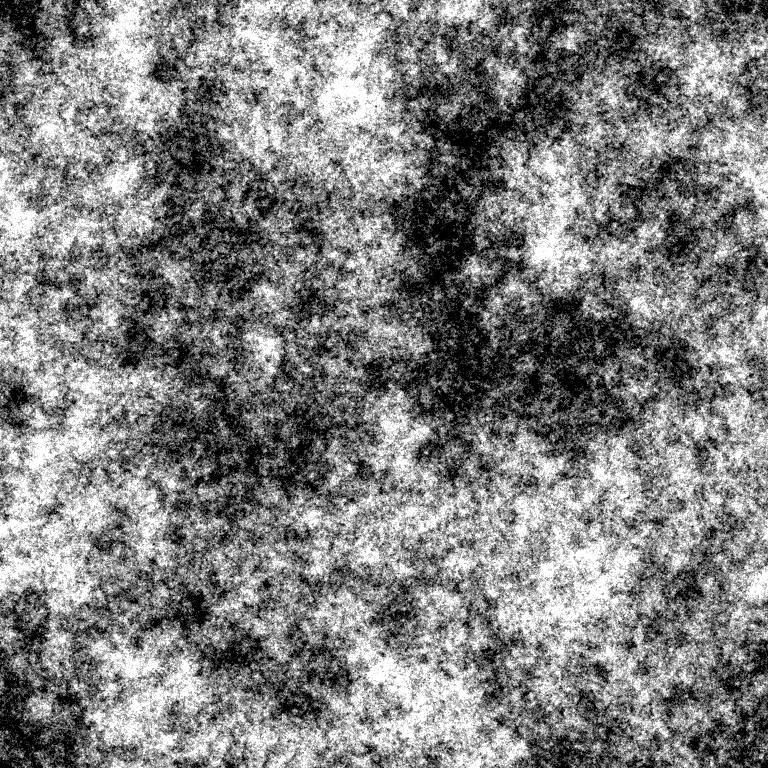
\includegraphics{multiscale.png}
\begin{verbatim}
plambda canvas randg | fft | plambda ':R /' | ifft | qauto - multiscale.png
\end{verbatim}

Comment: this is fractal or pink noise, obtained by forcing a spectral decay
of the form~$1/|\xi|$.

\section{Snowflakes}

\includegraphics{snowflakes.png}
\begin{verbatim}
plambda canvas ":x :y join 6 0 join cpow cimag :r 9 ^ / randc 3 ^ join" |\
	fft | plambda "halve cprod" | ifft | qeasy 2e17 5e17 - snowflakes.png
\end{verbatim}
Comment: this is a Cauchy-like white noise, filtered by the non-positive
kernel~$k(x,y) =
\frac{\mathrm{re}\left\{(x+iy)^6\right\}}{(x^2+y^2)^\frac{9}{2}}$, and a
threshold that keeps only the highest positive values.


\section{Dandelions}
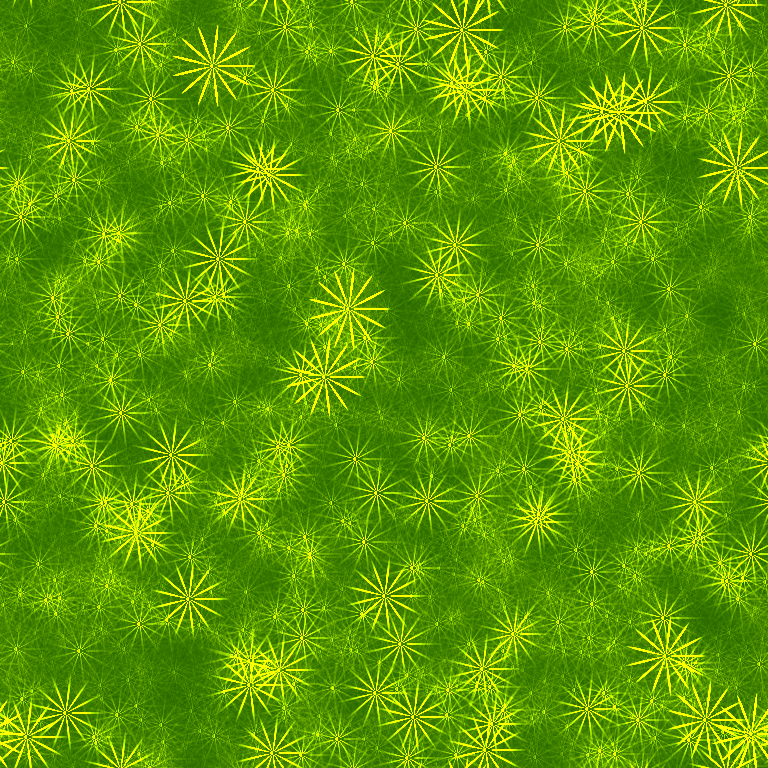
\includegraphics{dandelions.png}
\begin{verbatim}
KERNEL=':x :y join 13 0 join cpow creal :r 13.5 ^ / 3 fmax 3 -'
PALETTE='dup rot 128 2 / + 0 join3'
plambda canvas "$KERNEL randp join" | fft | plambda 'halve cprod' | ifft |\
	qeasy 0 3e4 | plambda - "$PALETTE" -o dandelions.png
\end{verbatim}
Comment: the same construction as \verb+snowflakes.png+ with a different
degree of polynomial and a green color palette.


\section{Heptachords}
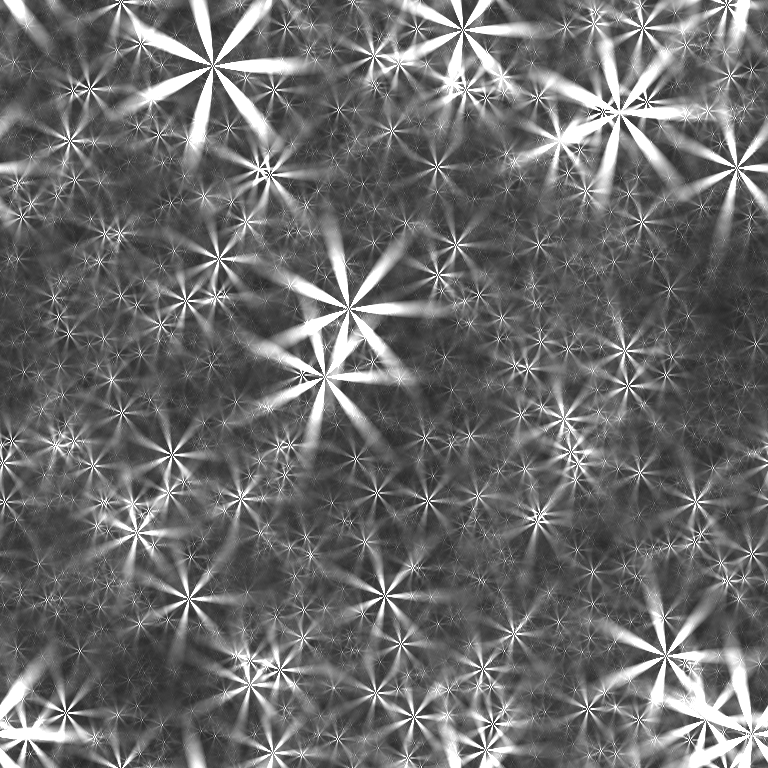
\includegraphics{heptachords.png}
\begin{verbatim}
KERNEL=':x :y join 7 0 join cpow creal :r 8 ^ / 3 fmax 3 -'
plambda canvas "$KERNEL randp join" | fft | plambda 'halve cprod' | ifft |\
	qeasy 1e5 9e5 - heptachords.png
\end{verbatim}
Comment: yet another polynomial kernel with a carefully selected contrast
change.


\section{Neurons}
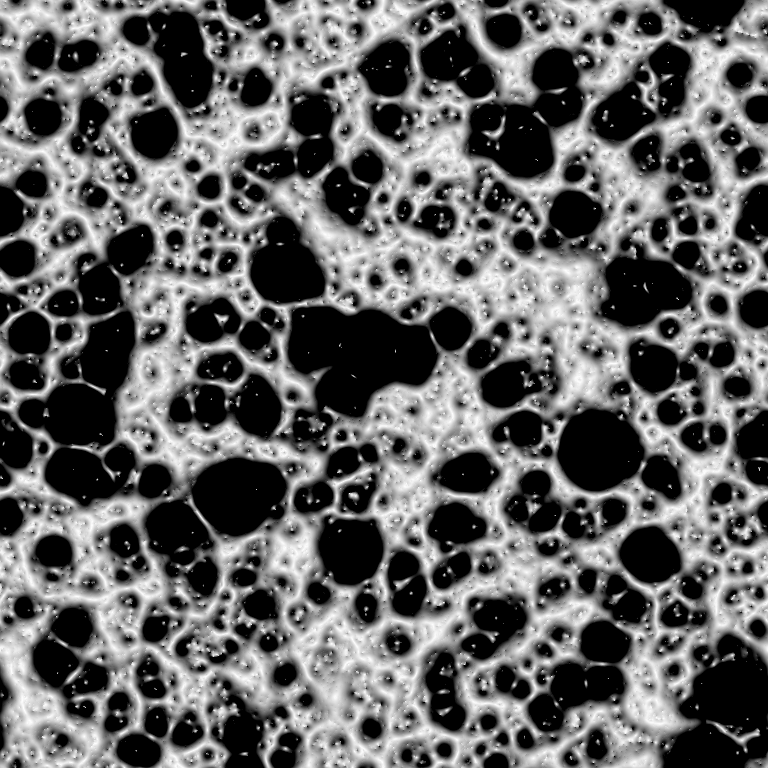
\includegraphics{neurons.png}
\begin{verbatim}
plambda canvas randp | blur l 10 | plambda 'x,nf' | qeasy 0.4 0 - neurons.png
\end{verbatim}
Comment: This is Pareto noise filtered by the derivative of Laplace kernel.
The final contrast change enhances the near-zero part of the image.

\section{Sponge}
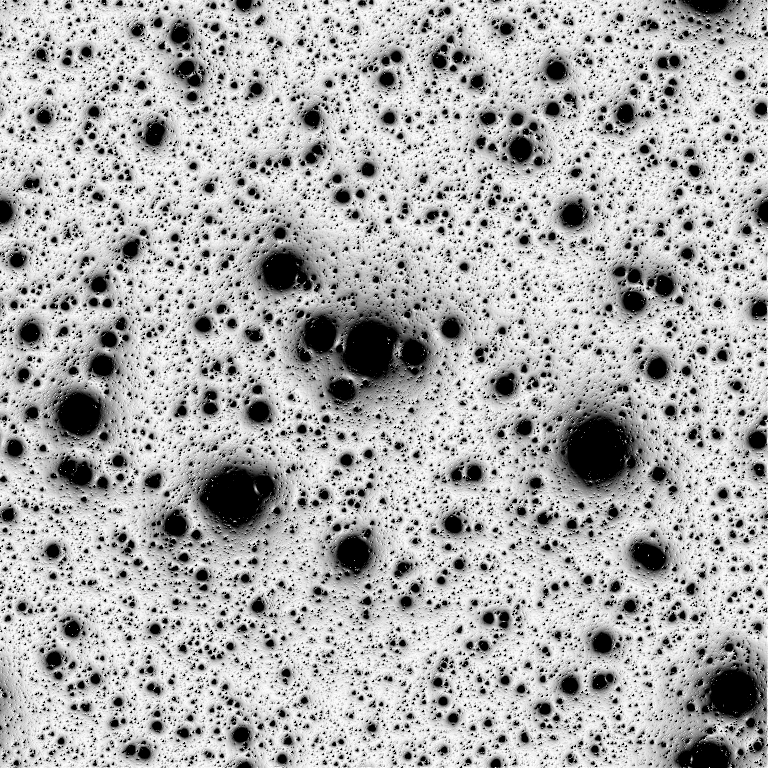
\includegraphics{sponge.png}
\begin{verbatim}
plambda canvas randp | blur i 0.3 | plambda 'x,nf' | qeasy 0.1 0 - sponge.png
\end{verbatim}
Comment: This is the same as \verb+neurons.png+, but using a Shepard instead
of a Laplacian kernel.

\section{Lava}
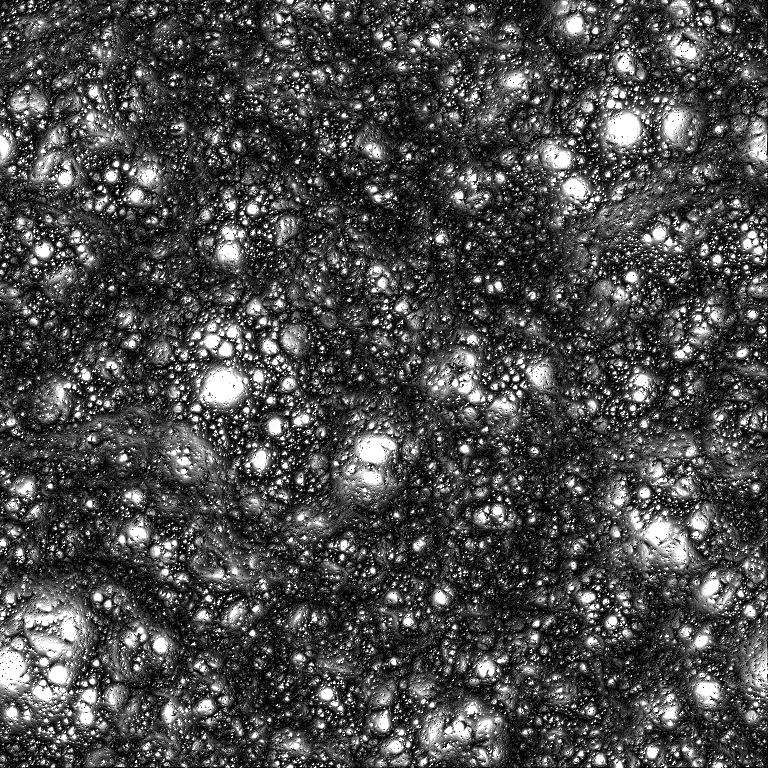
\includegraphics{lava.png}
\begin{verbatim}
plambda canvas 'randp randp randp join3' | blur i 0.3 | \
	plambda 'x,nf vmin' | qauto - lava.png
\end{verbatim}
Comment: Minimum of several instances of Pareto noise filtered by the
derivative of Shepard kernel.

\section{Folds}
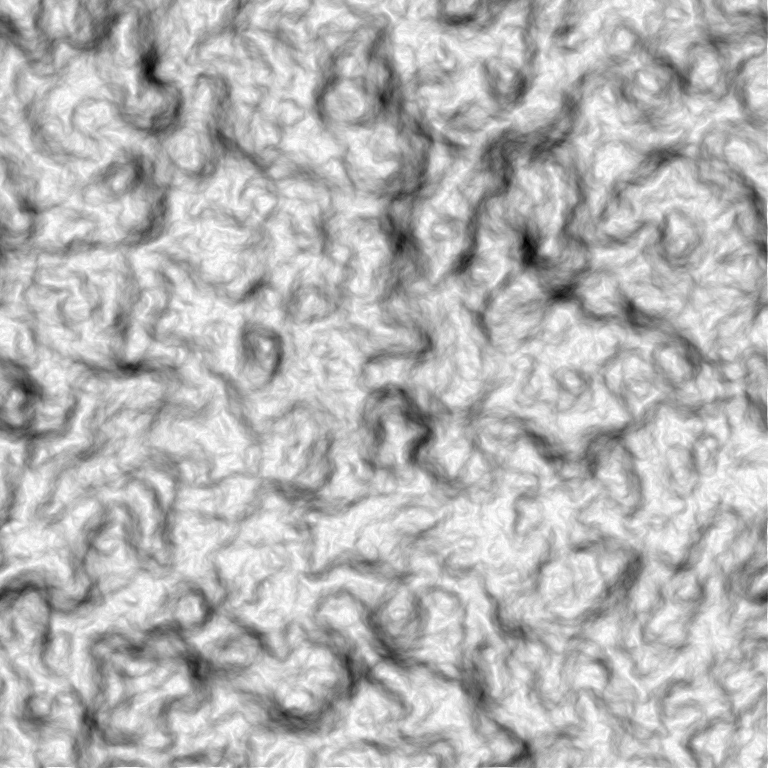
\includegraphics{folds.png}
\begin{verbatim}
plambda canvas randg | blur l 30 | plambda 'x,nf -1 *'|qauto -p 0 - folds.png
\end{verbatim}
Comment: this is white Gaussian noise blurred by the derivative of a large
Laplace kernel.  The resulting, nearly constant image, is then stretched to
span a visible dynamic range.

\section{Stucco}
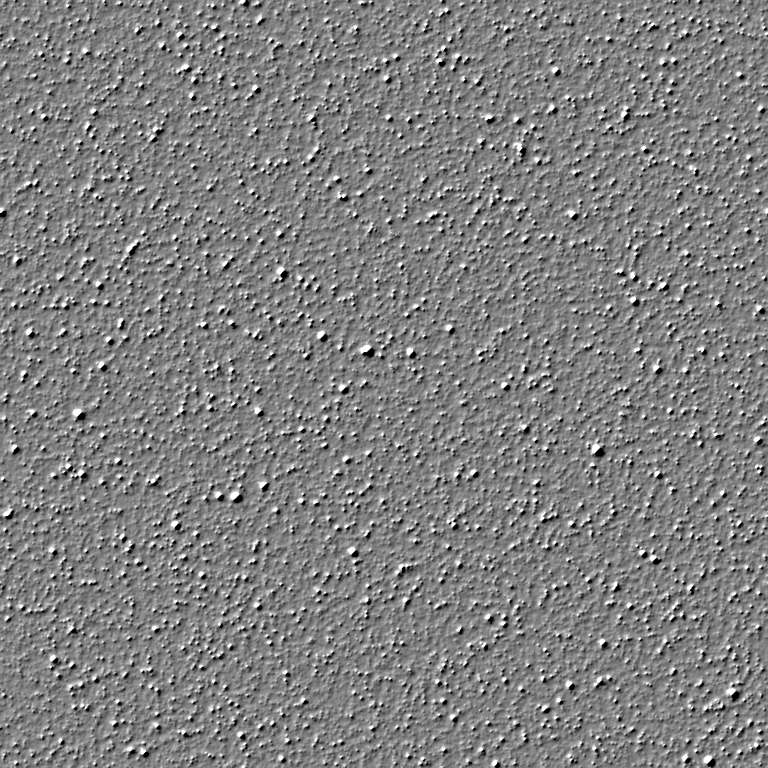
\includegraphics{stucco.png}
\begin{verbatim}
plambda canvas 'randp sqrt' | blur l 2 | plambda 'x,S' | qauto -p 1 - stucco.png
\end{verbatim}
Comment: this is the smoothed directional derivative of a high-variance white
noise.

\section{Blobs}
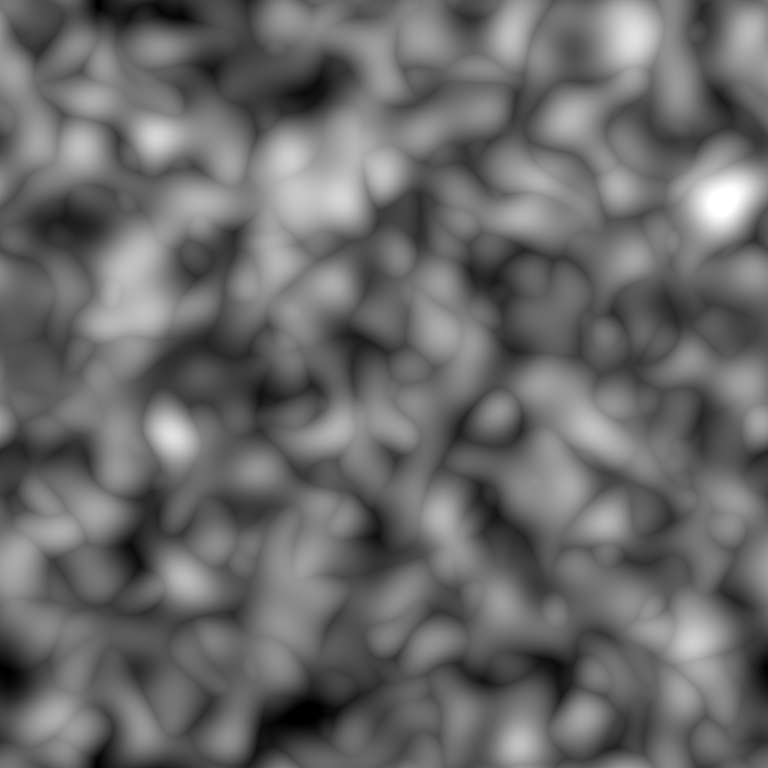
\includegraphics{blobs.png}
\begin{verbatim}
plambda canvas 'randu randu randu randu randu nstack njoin' | blur g 20 |\
	plambda vmax | qauto -p 0.1 - blobs.png
\end{verbatim}
Comment: this is the max of four Perlin noises.


%VSCRIPT wait

\section{Combined}
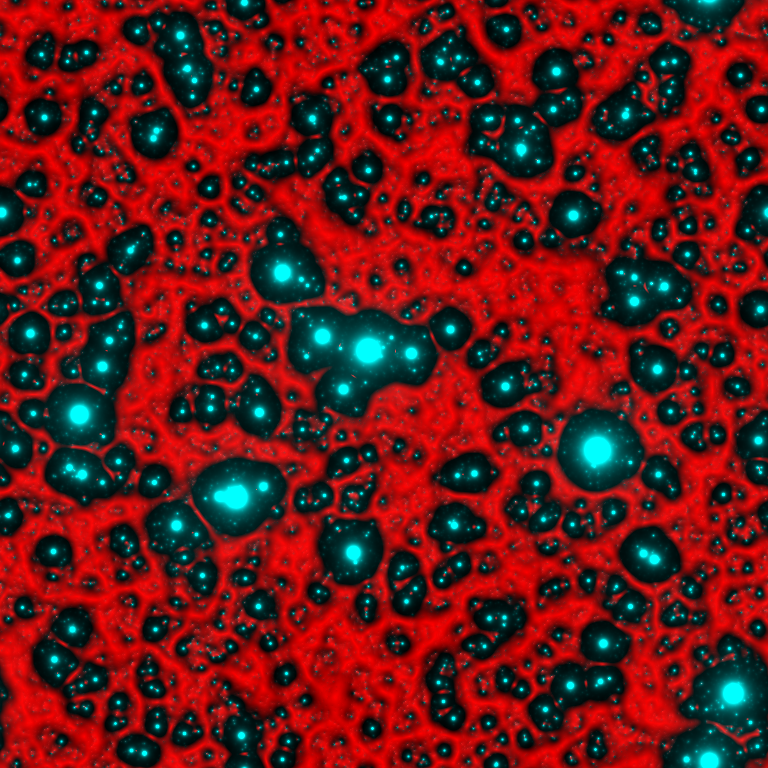
\includegraphics{combined.png}
\begin{verbatim}
plambda neurons.png starfield.png "dup join3" -o combined.png
\end{verbatim}
Comment: since many of the images above arise from exactly the same instance of
white noise, they are closely related.  Thus, they can be combined as
different channels of a color image to obtain funny effects.

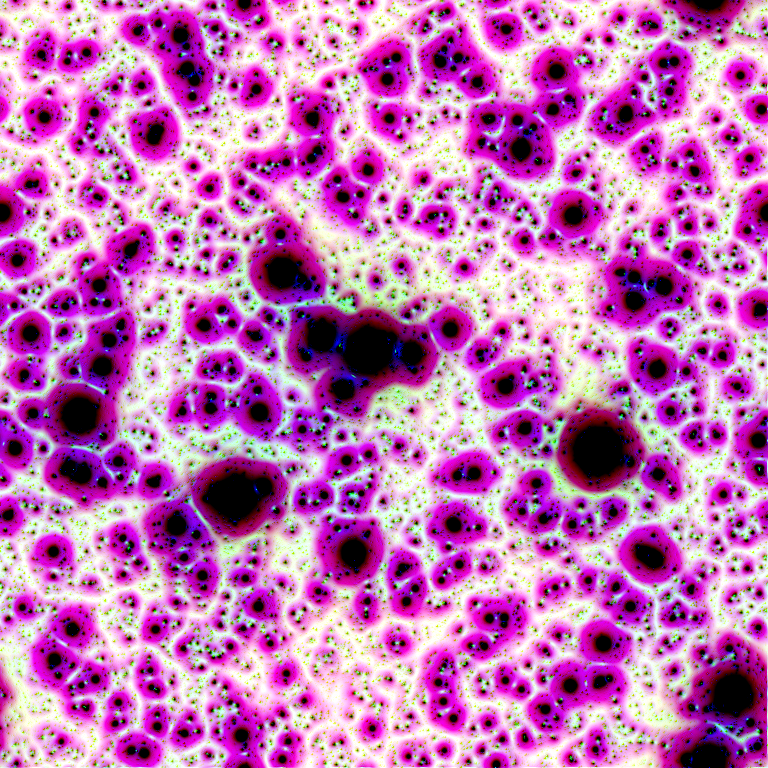
\includegraphics{combined2.png}
\begin{verbatim}
plambda starfield.png neurons.png sponge.png 'join3 -1 1 1 join3 *' |\
	qauto -i - combined2.png
\end{verbatim}
Comment: in color images, the choice of a color palette or another can have dramatic effects.

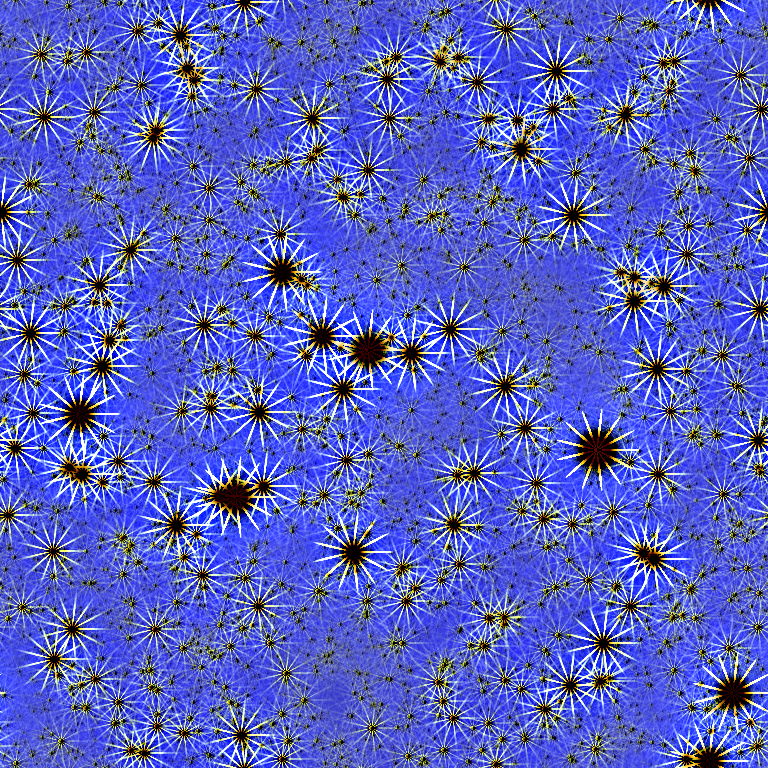
\includegraphics{comb3.png}
\begin{verbatim}
fftshift dandelions.png|plambda - starfield.png -|blur L 20|qauto -i - comb3.png
\end{verbatim}

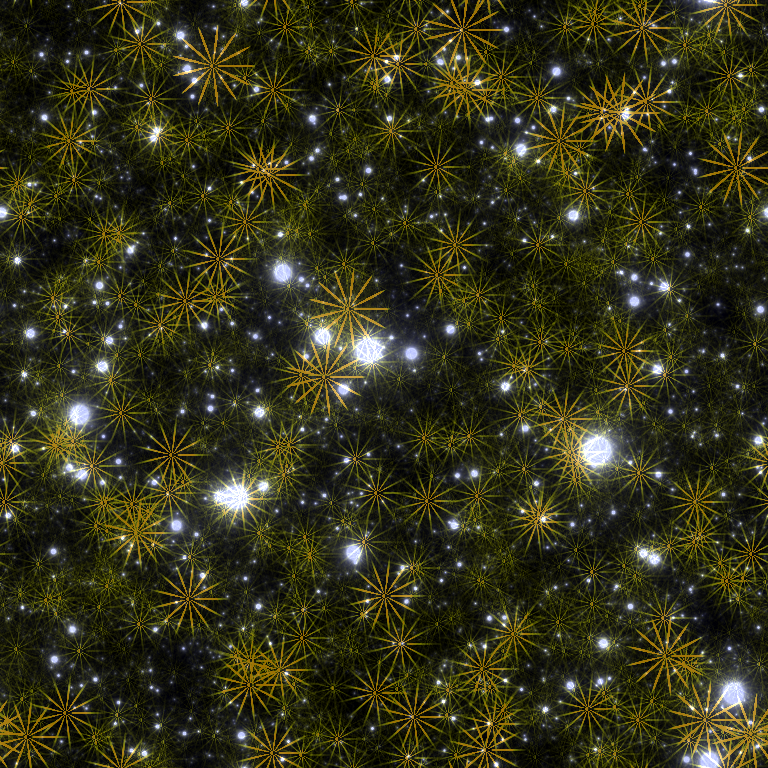
\includegraphics{combined4.png}
\begin{verbatim}
plambda dandelions.png starfield.png + | qauto -i -p 0.3 - combined4.png
\end{verbatim}
For unrelated images, the effect is less striking.










%{\bf Perlin noise} is Gaussian white noise smoothed using a Gaussian
%kernel.  This is the simplest posible case
%%SCRIPT plambda zero:256x256 randg | blur gauss  1 | qauto -p 1 - perlin1.png
%%SCRIPT plambda zero:256x256 randg | blur gauss  5 | qauto -p 1 - perlin5.png
%%SCRIPT plambda zero:256x256 randg | blur gauss 10 | qauto -p 1 - perlin10.png
%%SCRIPT plambda zero:256x256 randg | blur gauss 30 | qauto -p 1 - perlin30.png
%\begin{verbatim}
%plambda zero:256x256 randg | blur gauss  1 | qauto -p 1 - perlin1.png
%plambda zero:256x256 randg | blur gauss  5 | qauto -p 1 - perlin5.png
%plambda zero:256x256 randg | blur gauss 10 | qauto -p 1 - perlin10.png
%plambda zero:256x256 randg | blur gauss 30 | qauto -p 1 - perlin30.png
%\end{verbatim}
%\begin{tabular}{cccc}
%\includegraphics{perlin1.png}&
%\includegraphics{perlin5.png}&
%\includegraphics{perlin10.png}&
%\includegraphics{perlin30.png}\\
%	\verb+perlin1.png+ &
%	\verb+perlin5.png+ &
%	\verb+perlin10.png+ &
%	\verb+perlin30.png+ \\
%\end{tabular}
%
%{\bf Cauchy textures} are just like perlin noise, but changing all the
%Gaussians to Cauchys.  Since they have an extremely high dynamic range, their
%full power is unleashed by adjusting the contrast carefully.
%
%%SCRIPT plambda zero:256x256 randc | blur cauchy 1 | qauto -p 0.01 - cauchy1.png
%%SCRIPT plambda zero:256x256 randc | blur cauchy 1 | qauto -p 1  - cauchy2.png
%%SCRIPT plambda zero:256x256 randc | blur cauchy 1 | qauto -p 10 - cauchy3.png
%%SCRIPT plambda zero:256x256 randc | blur cauchy 1 | qauto -p 40 - cauchy4.png
%\begin{verbatim}
%plambda zero:256x256 randc | blur cauchy 1 | qauto -p 0.01 - cauchy1.png
%plambda zero:256x256 randc | blur cauchy 1 | qauto -p 0.1 - cauchy2.png
%plambda zero:256x256 randc | blur cauchy 1 | qauto -p 10 - cauchy3.png
%plambda zero:256x256 randc | blur cauchy 1 | qauto -p 30 - cauchy4.png
%\end{verbatim}
%\begin{tabular}{cccc}
%\includegraphics{cauchy1.png}&
%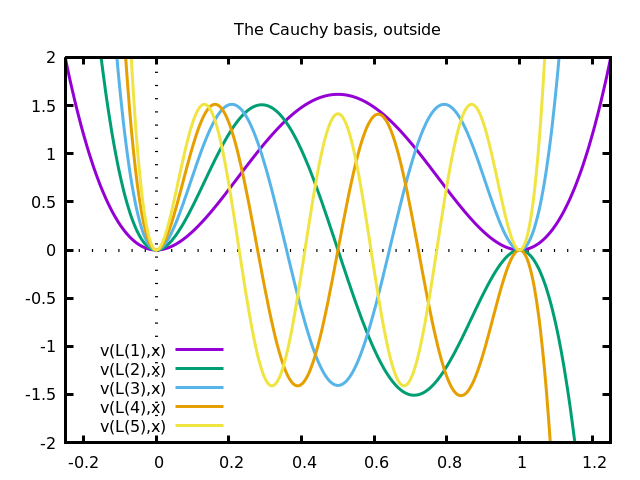
\includegraphics{cauchy2.png}&
%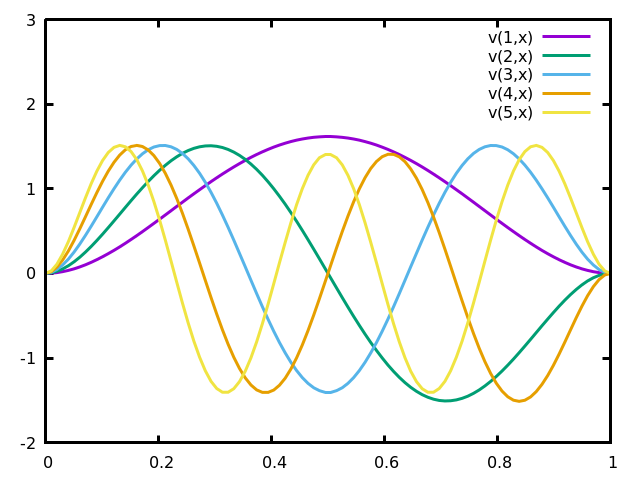
\includegraphics{cauchy3.png}&
%\includegraphics{cauchy4.png}\\
%	\verb+cauchy1.png+ &
%	\verb+cauchy2.png+ &
%	\verb+cauchy3.png+ &
%	\verb+cauchy4.png+ \\
%\end{tabular}
%
%{\bf Pareto textures} are just like perlin noise, but changing all the
%Gaussians to Paretos.  Since they have an extremely high dynamic range, their
%full power is unleashed by adjusting the contrast carefully.
%
%%SCRIPT plambda zero:256x256 randp | blur pareto 0.31 | qauto -p 0.01 - pareto1.png
%%SCRIPT plambda zero:256x256 randp | blur pareto 0.31 | qauto -p 1  - pareto2.png
%%SCRIPT plambda zero:256x256 randp | blur pareto 0.31 | qauto -p 10 - pareto3.png
%%SCRIPT plambda zero:256x256 randp | blur pareto 0.31 | qauto -p 40 - pareto4.png
%\begin{verbatim}
%plambda zero:256x256 randp | blur a 1 | qauto -p 0.01 - pareto1.png
%plambda zero:256x256 randp | blur a 1 | qauto -p 0.1 - pareto2.png
%plambda zero:256x256 randp | blur a 1 | qauto -p 10 - pareto3.png
%plambda zero:256x256 randp | blur a 1 | qauto -p 30 - pareto4.png
%\end{verbatim}
%\begin{tabular}{cccc}
%\includegraphics{pareto1.png}&
%\includegraphics{pareto2.png}&
%\includegraphics{pareto3.png}&
%\includegraphics{pareto4.png}\\
%	\verb+pareto1.png+ &
%	\verb+pareto2.png+ &
%	\verb+pareto3.png+ &
%	\verb+pareto4.png+ \\
%\end{tabular}

\section{Appendix: Technical details}

The programs required to run these scripts are available in \verb+imscript+:
\url{http://github.com/mnhrdt/imscript}.

Here are the help messages of the four main programs:

{\bf qauto}
 \begin{verbatim}
Qauto quantizes an image into [0,255].

The image is trasformed by an affine contrast change I -> a*I + b
and then the colors are saturated and quantized into [0,255].
The parameters (a,b) of the contrast change are computed to statisfy
certain conditions. By default, they are chosen so that 5% of the pixels
are saturated.

Usage: qauto in.tiff out.png
   or: qauto in.tiff > out.pnm
   or: cat in.tiff | qauto > out.pnm

Options:
 -p X      use a percentile of X% (default X=5)
 -f        do not quantize the output, only rescale the values
 -i        treat each pixel dimension independently
 -h        display short help message
 --help    display longer help message

Examples:
 qauto in.tiff out.png          Quantize an image by simplest color balance.
 qauto -i in.png out.png        Remove color biases
 \end{verbatim}

{\bf blur}
 \begin{verbatim}
Blur convolves the input image by the requested positive kernel.
Only the first letter of the kernel name is considered.
If the name of the kernel is uppercase, it subtracts the result
from the original image.

Usage: blur KERNEL SIZE in.tiff out.tiff
   or: blur KERNEL SIZE in.tiff > out.tiff
   or: cat in.tiff | blur KERNEL SIZE > out.tiff

Kernels:
 square   a square block of the given radius
 disk     a rasterized disk of the given radius
 gauss    a Gaussian kernel of the given variance
 laplace  a Laplace kernel of the given variance
 cauchy   a Cauchy kernel of the given scale
 q        Log-cauchy kernel
 u        "good-cauchy"
 p        powerlaw
 a        pareto
 i        inverse distance (useful for Shepard interpolation)
 y        inverse distance (with different parameter normalization)
 r        Land
 z        inverse log-distance
 t        r^2 log(r)  (useful for biharmonic interpolation)
 o        log(r)

Options:
 -z        zero boundary
 -s        symmetrized boundary
 -p        periodic boundary

Examples:
 blur g 1.6                              Smooth an image by a slight amount
 blur C 1 | qauto                        Linear retinex
 plambda - "x,l -1 *" | blur i 0.25      Laplacian square root
 plambda - "x,l" | blur z 0.25 | plambda - "0 >"      Linear dithering
 \end{verbatim}

{\bf plambda}
 \begin{verbatim}
Plambda evaluates an expression with images as variables.

The expression is written in reverse polish notation using common
operators and functions from `math.h'.  The variables appearing on the
expression are assigned to each input image in alphabetical order.

EXPRESSIONS:

A "plambda" expression is a sequence of tokens.
Tokens may be constants,
variables, or operators.  Constants and variables get their value
computed and pushed to the stack.  Operators pop values from the stack,
apply a function to them, and push back the results.

CONSTANTS: numeric constants written in scientific notation, and "pi"

OPERATORS: +, -, *, ^, /, <, >, ==, and all the functions from math.h

LOGIC OPS: if, and, or, not

VARIABLES: anything not recognized as a constant or operator.  There
must be as many variables as input images, and they are assigned to
images in alphabetical order.  If there are no variables, the input
images are pushed to the stack.

All operators (unary, binary and ternary) are vectorizable.  Thus, you can
add a scalar to a vector, divide two vectors of the same size, and so on.
The semantics of each operation follows the principle of least surprise.

Some "sugar" is added to the language:

Predefined variables (always preceeded by a colon):
 :i	horizontal coordinate of the pixel
 :j	vertical coordinate of the pixel
 :w	width of the image
 :h	heigth of the image
 :n	number of pixels in the image
 :x	relative horizontal coordinate of the pixel
 :y	relative horizontal coordinate of the pixel
 :r	relative distance to the center of the image
 :t	relative angle from the center of the image
 :I	horizontal coordinate of the pixel (centered)
 :J	vertical coordinate of the pixel (centered)
 :P	horizontal coordinate of the pixel (phased)
 :Q	vertical coordinate of the pixel (phased)
 :R	centered distance to the center
 :L	minus squared centered distance to the center
 :W	width of the image divided by 2*pi
 :H	height of the image divided by 2*pi

Variable modifiers acting on regular variables:
 x		value of pixel (i,j)
 x(0,0)		value of pixel (i,j)
 x(1,0)		value of pixel (i+1,j)
 x(0,-1)	value of pixel (i,j-1)
 x[0]		value of first component of pixel (i,j)
 x[1]		value of second component of pixel (i,j)
 x(1,2)[3]	value of fourth component of pixel (i+1,j+2)

Comma modifiers (pre-defined local operators):
 a,x	x-derivative of the image a
 a,y	y-derivative
 a,xx	second x-derivative
 a,yy	second y-derivative
 a,xy	crossed second derivative
 a,l	Laplacian
 a,g	gradient
 a,n	gradient norm
 a,d	divergence
 a,S	shadow operator
 a,xf	x-derivative, forward differences
 a,xb	x-derivative, backward differences
 a,xc	x-derivative, centered differences
 a,xs	x-derivative, sobel
 a,xp	x-derivative, prewitt
 etc

Stack operators (allow direct manipulation of the stack):
 del	remove the value at the top of the stack (ATTTOS)
 dup	duplicate the value ATTTOS
 rot	swap the two values ATTTOS
 split	split the vector ATTTOS into scalar components
 join	join the components of two vectors ATTOTS
 join3	join the components of three vectors ATTOTS
 njoin	join the components of n vectors
 halve	split an even-sized vector ATTOTS into two equal-sized parts
 nstack	current number of elements in the stack (useful with njoin)

Magic variable modifiers (global data associated to each input image):
 x%i	value of the smallest sample of image x
 x%a	value of the largest sample
 x%v	average sample value
 x%m	median sample value
 x%s	sum of all samples
 x%I	value of the smallest pixel (in euclidean norm)
 x%A	value of the largest pixel
 x%V	average pixel value
 x%S	sum of all pixels
 x%Y	component-wise minimum of all pixels
 x%E	component-wise maximum of all pixels
 x%qn	nth sample percentile
 x%On	component-wise nth percentile
 x%Wn	component-wise nth millionth part
 x%0n	component-wise nth order statistic
 x%9n	component-wise nth order statistic (from the right)

Random numbers (seeded by the SRAND environment variable):
 randu	push a random number with distribution Uniform(0,1)
 randn	push a random number with distribution Normal(0,1)
 randc	push a random number with distribution Cauchy(0,1)
 randl	push a random number with distribution Laplace(0,1)
 rande	push a random number with distribution Exponential(1)
 randp	push a random number with distribution Pareto(1)
 rand	push a random integer returned from rand(3)

Vectorial operations (acting over vectors of a certain length):
 topolar	convert a 2-vector from cartesian to polar
 frompolar	convert a 2-vector from polar to cartesian
 hsv2rgb	convert a 3-vector from HSV to RGB
 rgb2hsv	convert a 3-vector from RGB to HSV
 xyz2rgb	convert a 3-vector from XYZ to RGB
 rgb2xyz	convert a 3-vector from RGB to XYZ
 cprod		multiply two 2-vectrs as complex numbers
 cexp		complex exponential
 cpow		complex power
 mprod		multiply two 2-vectrs as matrices (4-vector = 2x2 matrix, etc)
 vprod		vector product of two 3-vectors
 sprod		scalar product of two n-vectors
 mdet		determinant of a n-matrix (a n*n-vector)
 mtrans		transpose of a matrix
 mtrace		trace of a matrix
 minv		inverse of a matrix
 vavg		average value of a vector
 vsum		sum of the components of a vector
 vmul		product of the components of a vector
 vmax		max component of a vector
 vmin		min component of a vector
 vnorm		euclidean norm of a vector
 vdim		length of a vector

Registers (numbered from 1 to 9):
 >7	copy to register 7
 <3	copy from register 3

Usage: plambda a.png b.png c.png ... "EXPRESSION" > output
   or: plambda a.png b.png c.png ... "EXPRESSION" -o output.png
   or: plambda -c num1 num2 num3  ... "EXPRESSION"

Options:
 -o file	save output to named file
 -c		act as a symbolic calculator
 -h		display short help message
 --help		display longer help message

Examples:
 plambda a.tiff b.tiff "x y +" > sum.tiff    Compute the sum of two images.
 plambda -c "1 atan 4 *"                     Print pi
 plambda -c "355 113 /"                      Print an approximation of pi
 \end{verbatim}


% vim:set tw=800 filetype=tex spell spelllang=en:
